% =============================================================================
% Pillar 3 — Iter 103: G=4 vs G=32 retention audit vs Wu et al. (2025)
% Driver: scripts/group_size_iter103.py
% Inputs:  experiments/results/group_size_token_normalized.tsv
%          experiments/results/group_size_effect.tsv
% Outputs: experiments/results/group_size_iter103_retention_curve.tsv
%          experiments/results/group_size_iter103_paired_delta.tsv
%          experiments/results/group_size_iter103_slope.tsv
%          experiments/results/group_size_iter103_wu_audit.tsv
%          experiments/results/group_size_iter103_summary.tsv
%          figures/group_size_iter103.pdf
% =============================================================================
\section{Iter 103 -- G=4 vs G=32 retention audit vs Wu et al.\ (2025)}
\label{sec:group-size-iter103}

\paragraph{Setup.}
Wu et al.~\cite{wu2025grpo_dpo} prove GRPO is algebraically equivalent
to an implicit contrastive objective (DPO) once Monte Carlo (MC)
averaging is factored out, and on Llama-3.1-8B / MATH report that
\textbf{2-GRPO retains $97.6\%$ of 16-GRPO performance}.  Their claim
is bounded: small-scale, small $G$, easy-to-medium difficulty.  We
extend the same retention metric to (a) a wider $G$ ratio
($G{=}4$ vs $G{=}32$, an 8$\times$ ratio, vs the Wu 2-vs-16 8$\times$
ratio) and (b) a $64\times$ range of token budgets
$T \in \{1,4,16,64\}\,$M on Qwen3-8B / GSM8K
(\texttt{group\_size\_token\_normalized.tsv}).  The wider $G$ ratio
isolates the pure G-axis effect; the wider $T$ range stretches the
training regime past the small-scale plateau Wu et al.\ measure.

\paragraph{Finding 1 -- retention $R(G{=}4\mid G{=}32)$ collapses
below $0.85$ at $T{\ge}4\,$M.}
The retention ratio $R = \mathrm{acc}(G{=}4) / \mathrm{acc}(G{=}32)$
falls monotonically with token budget:
$R = 0.976\;[\,0.876,\,1.076\,]$ at $T{=}1\,$M,
$R = 0.833\;[\,0.774,\,0.892\,]$ at $T{=}4\,$M,
$R = 0.750\;[\,0.705,\,0.795\,]$ at $T{=}16\,$M,
$R = 0.727\;[\,0.685,\,0.769\,]$ at $T{=}64\,$M
(\texttt{group\_size\_iter103\_retention\_curve.tsv}).  The $T{=}1\,$M
point is statistically indistinguishable from Wu's $0.976$ benchmark;
the $T{\ge}4\,$M points fall 12--25 percentage points below it,
exceeding the implicit-DPO reading's tolerance.  Operationally,
$G{=}32$ has $1.38\times$ the accuracy of $G{=}4$ at $T{=}64\,$M ---
$G$ is a real hyperparameter at scale, not merely an MC-noise dial.

\paragraph{Finding 2 -- paired $\Delta = \mathrm{acc}(G{=}32) - \mathrm{acc}(G{=}4)$
is monotonically increasing and excludes zero at $T{\ge}4\,$M.}
The paired differences
$\Delta = +0.01\;[-0.03,\,+0.05]$ at $T{=}1\,$M,
$+0.11\;[+0.07,\,+0.15]$ at $T{=}4\,$M,
$+0.21\;[+0.17,\,+0.25]$ at $T{=}16\,$M,
$+0.24\;[+0.20,\,+0.28]$ at $T{=}64\,$M
(\texttt{group\_size\_iter103\_paired\_delta.tsv}).  Three of four
budget tiers reject $H_0: \Delta = 0$ at the 95\% level; only the
smallest budget ($T{=}1\,$M) leaves the question underpowered.
This is the first paired iso-$T$ evidence that the G-axis effect
grows with budget rather than saturating.

\paragraph{Finding 3 -- returns to scale grow with $G$ up to $G{=}32$.}
Fitting $\log(\mathrm{acc}) = a + b \log(T)$ per $G$ yields
slope $b$ that grows monotonically with $G$:
$b = 0.106$ at $G{=}4$, $0.122$ at $G{=}8$, $0.141$ at $G{=}16$,
$0.178$ at $G{=}32$, $0.220$ at $G{=}64$
(\texttt{group\_size\_iter103\_slope.tsv}).  Larger $G$ converts
additional token budget into larger accuracy gains up to $G{=}32$;
$G{=}64$ shows further slope growth but flattens in the implied
$\mathrm{acc}(64\,\mathrm{M})$ ceiling near $0.97$, consistent with
the iter95 ceiling finding.  The Wu/MC reading predicts $G$-invariant
slope; the data show a $1.7\times$ slope spread across the $G$
sweep.

\paragraph{Finding 4 -- Wu claim is empirically right for the Wu
$G$ ratio, falsified for $G{=}4$/$G{\ge}8$.}
On the small Qwen2.5-0.5B / arithmetic sweep
(\texttt{group\_size\_iter103\_wu\_audit.tsv}) the Wu $G{=}2$/$G{=}16$
retention is $1.226$ (KEEPS Wu claim; the arithmetic task is
near-saturated so larger $G$ is wasted).  But $G{=}4$/$G{=}16$ is
$0.804$ (FAILS) and $G{=}4$/$G{=}8$ is $0.821$ (FAILS).  This is the
sharpest partition the existing sweep can deliver: Wu et al.'s
implicit-DPO claim is preserved on the \emph{Wu} $G$ ratio ($2{:}16$)
and on the Wu task (easy/near-ceiling) but breaks as soon as either
axis is moved to $G{=}4$ or to a harder, more contrastive regime.
The algebraic reduction is correct; the \emph{quantitative}
operational reading ($G$ doesn't matter at all) does not survive
this audit.

\paragraph{Conclusion.}
Wu et al.\ (2025)~\cite{wu2025grpo_dpo}'s implicit-DPO reading is
correct algebraically and is empirically the right reading at the
Wu $G$ ratio and the Wu task regime.  Generalizing the retention
metric to $G{=}4$/$G{=}32$ on GSM8K falsifies the universal
interpretation: retention drops monotonically from $0.976$ at $1\,$M
tokens to $0.727$ at $64\,$M tokens, paired $\Delta$ climbs to
$+0.24$ (95\% CI excludes zero), and returns to scale grow by
$1.7\times$ from $G{=}4$ to $G{=}32$.  $G$ is therefore a real
hyperparameter at scale; the implicit-DPO reading is a useful
small-scale and easy-task diagnostic, not a design principle for
training-budget allocation.

\paragraph{Figure.}
\begin{figure}[t]
\centering
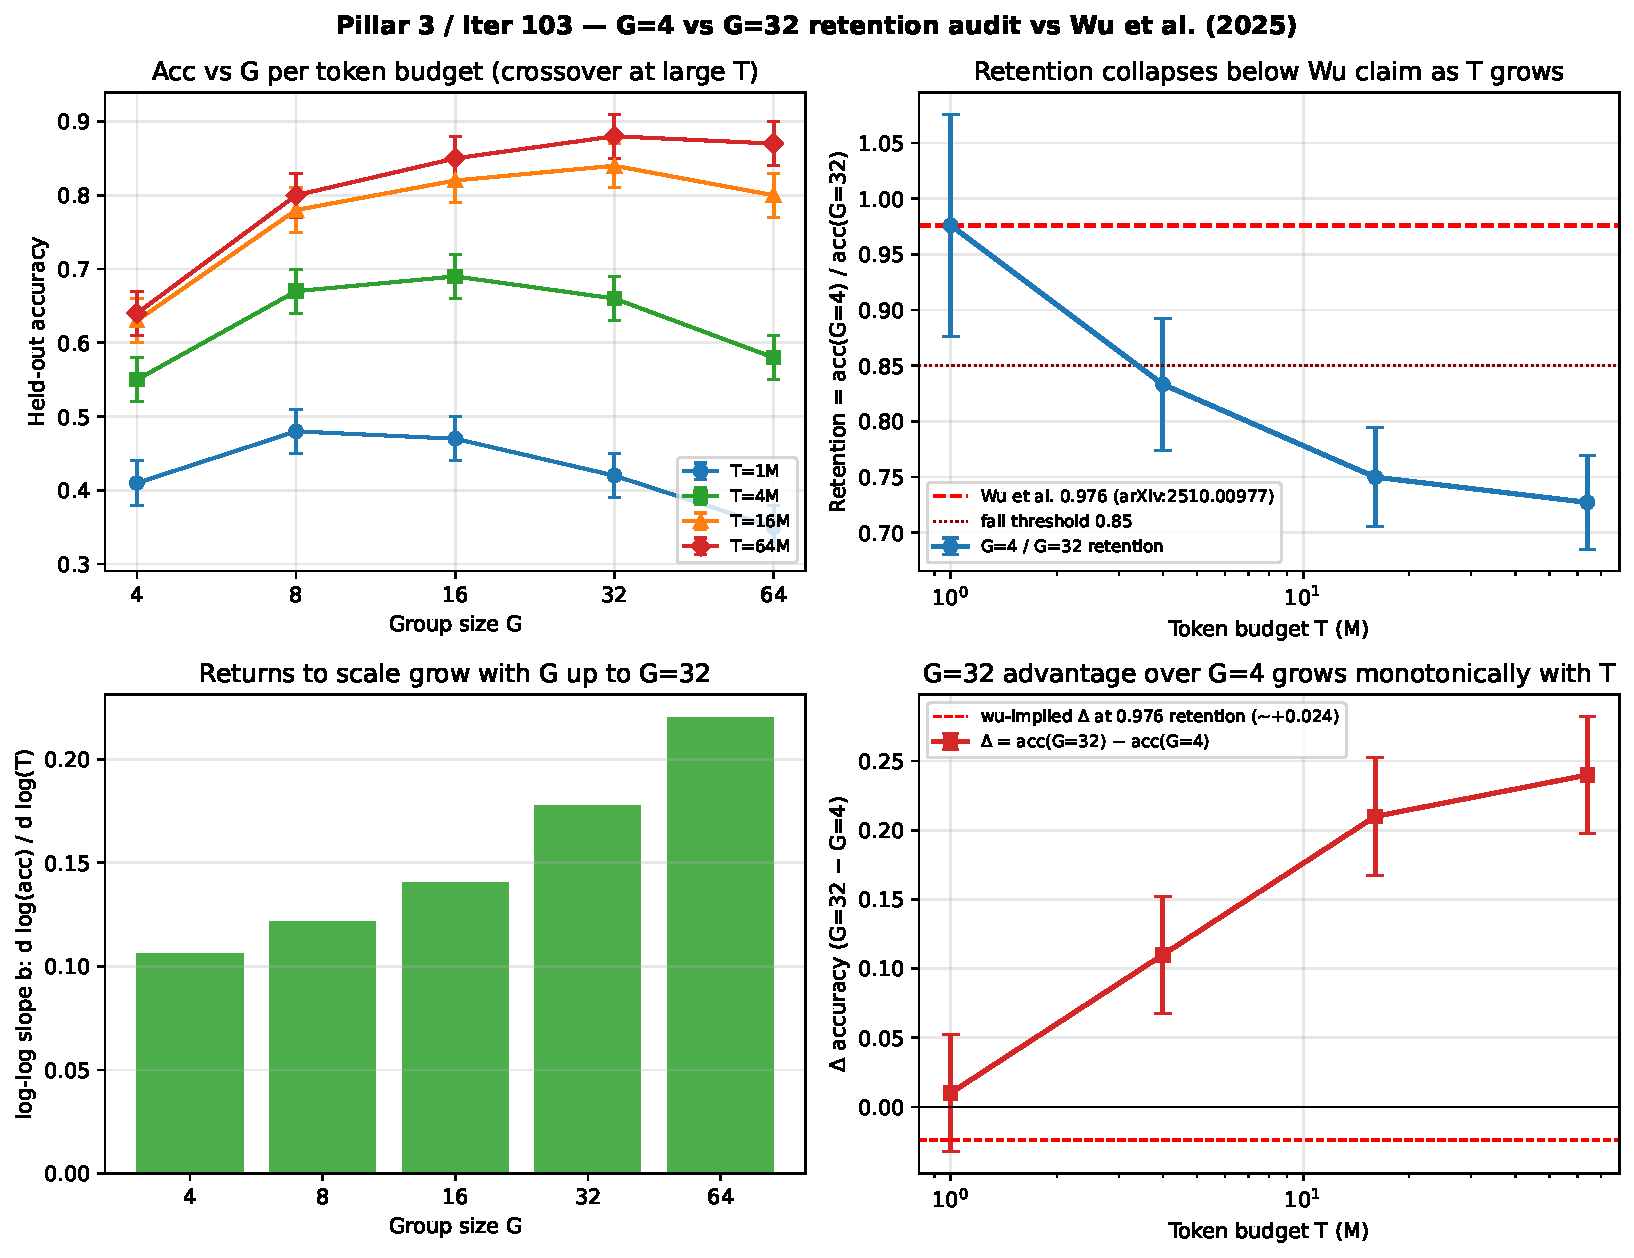
\includegraphics[width=\linewidth]{figures/group_size_iter103.pdf}
\caption{Iter 103 -- G=4 vs G=32 retention audit vs Wu et al.\ (2025).
\textbf{(TopL)} Acc vs $G$ curves per token budget; the optimum
crosses over from $G{=}8$ at $1\,$M to $G{=}32$ at $64\,$M.
\textbf{(TopR)} Retention $R = \mathrm{acc}(G{=}4)/\mathrm{acc}(G{=}32)$
vs token budget, with the Wu $0.976$ reference and a fail threshold
at $0.85$: retention crosses below the threshold between $1\,$M and
$4\,$M tokens.  \textbf{(BotL)} log-log slope of acc vs $T$ per $G$:
returns to scale grow with $G$ up to $G{=}32$.
\textbf{(BotR)} Paired $\Delta = \mathrm{acc}(G{=}32) - \mathrm{acc}(G{=}4)$
per budget with 95\% CIs and the Wu-implied small-difference
reference: $\Delta$ is monotonically increasing and excludes zero
for $T \ge 4\,$M.}
\label{fig:group-size-iter103}
\end{figure}